\section{Introduction}
\label{chap:introduction}

As students, we are constantly seeking opportunities to maximise our limited budgets. 
One area where we identified potential for cost savings is air travel, particularly during peak travel times such as holidays. 
During these periods, ticket prices can increase significantly, making it challenging for us to afford travel for visiting family or taking vacations.

With this in mind, we decided to undertake a project to develop a model capable of predicting the prices of round-trip tickets from Lufthansa and Swiss airlines to São Paulo and New York City.
By analysing historical data on ticket prices and other relevant factors such as holidays, we aim to identify patterns and trends that can assist us in forecasting future ticket prices.
Utilising this information, our goal is to determine the optimal time to purchase a ticket for each destination, allowing us to save money and make the most of our travel budget.

Through this project, we hope to gain valuable experience in working with time series data and developing predictive models while also discovering practical ways to save money on air travel during peak travel times.
By focusing on two specific airlines and destinations, we aim to develop a model that is both accurate and applicable to our travel needs.

\subsection{Research questions/hypotheses}
\label{sec:quesstion}

The objective of this study is to create a model that can predict the prices of round-trip tickets for Lufthansa and Swiss flights to Sao Paulo and NYC. 
The first hypothesis posits that historical ticket prices for these flights exhibit identifiable patterns and trends. 
By examining ticket price data over time, it is anticipated that these patterns can be discerned and used to forecast future prices. 
To evaluate this hypothesis, historical ticket price data and other relevant factors will be analyzed to identify patterns and trends. 
This analysis will employ statistical methods to reveal relationships between ticket prices and other variables such as the time at which flight ticket data is collected.

The second hypothesis proposes that the time at which flight ticket data is collected significantly impacts ticket prices.
It is anticipated that collecting data at certain times during the week will result in lower ticket prices.

The third hypothesis asserts that a model trained on historical data can accurately predict future ticket prices. 
To test these hypotheses, a predictive model will be created using machine learning techniques to forecast future ticket prices based on historical data.
This model will consider a variety of factors known to affect ticket prices, including the time at which flight ticket data is collected and airline-specific factors.

The research questions are: What are the primary factors that influence ticket prices for Lufthansa and Swiss flights to Sao Paulo and NYC? How does the time at which flight ticket data is collected impact ticket prices? When is the optimal time to collect flight ticket data to minimize cost? And how accurately can future ticket prices be predicted using a model trained on historical data?
In order to answer these questions, the study will involve collecting and analyzing large amounts of data on ticket prices and other relevant factors. This data will be used to train and evaluate the predictive model, allowing us to determine its accuracy and effectiveness in forecasting future ticket prices. By identifying the key factors that influence ticket prices and determining the optimal time to collect flight ticket data, we hope to provide valuable insights for travelers looking to save money on air travel.


\section{Data}
\label{chap:data}
In this project, data was collected from the online travel booking platform booking.com.
This platform was chosen due to its extensive coverage of flights from Lufthansa and Swiss airlines to Sao Paulo and NYC.
Data collection was conducted on a daily basis, with observations recorded every 2 hours between 8 am and 10 pm.
This schedule was chosen to capture variations in ticket prices throughout the day.
In total, 11619 data points were collected over the course of the project.

The data collected includes a range of variables relevant to the research questions.
These include the price for round-trip tickets for the specified destinations using Lufthansa and Swiss airlines,
as well as the departure and arrival times/dates for both the outbound and inbound flights.
Additionally, data on the duration of the outbound and inbound flights and the number of stopovers for both flights were recorded.
Since the weight allowance for luggage is consistent across both airlines, this variable was not included in the data collection.

Furthermore, the time at which each observation was recorded was also noted in order to facilitate analysis of trends in ticket prices relative to the day/time of the week.
This information is expected to provide valuable insights into how ticket prices vary over time.

By analyzing this comprehensive dataset, it is anticipated that patterns and trends can be identified that will aid in predicting future ticket prices for these specific airlines and destinations.
The data collected will be used to train a predictive model that can forecast future ticket prices with a high degree of accuracy.
This model will be a valuable tool for travelers seeking to minimize costs and maximize their travel budgets.

\subsection{Data preparation}
\label{sec:data}
The initial phase of the methodology involves collecting data on ticket prices for Lufthansa and Swiss flights to Sao Paulo and New York City.
This objective is achieved by utilizing the Selenium web automation tool to extract ticket price data from the airlines’ websites.
Selenium is a robust tool that facilitates the automation of web browser interactions, enabling the visiting of websites, inputting flight information, and retrieving ticket price data in an automated fashion.

Data collection occurs at regular intervals, with ticket price data being collected every 2 hours from 8 am to 10 pm daily.
This frequent data collection captures changes in ticket prices over time, providing a rich dataset for analysis.

Once the data has been collected, it is converted into a structured format using CSV (Comma-Separated Values) files.
The data for each destination is stored in separate folders: one for flights from Brussels to Sao Paulo ($bxl\_to\_sao$) and one for flights from Brussels to New York City ($bxl\_to\_nyc$).
Each CSV file contains information on ticket prices, flight dates, and other relevant factors.

Furthermore, the collected data is cleaned using the Pandas library in Python.
This process includes checking the data for missing or incorrect values and ensuring that it has been correctly collected for the chosen destinations and airlines.
The cleaned data is then stored in data frames, which are two-dimensional data structures that enable easy manipulation and analysis of the data.

After cleaning the data, it is preprocessed to prepare it for analysis. This step involves transforming the data into a format that can be easily analyzed.
For example, categorical variables may be converted into numerical values or the data may be normalized to ensure that all variables are on a similar scale.
By cleaning and preprocessing the data, its accuracy is ensured and it is ready for analysis.
This enables identification of patterns and trends in the data, which form the basis of a predictive model.
By using tools such as Pandas and Python, large amounts of data can be efficiently manipulated and analyzed.

\subsection{Data visualizations}
\label{sec:data}

In our analysis of flight prices, we used the Seaborn, plotnine and Matplotlib libraries in Python to create visualizations of our data.
These powerful tools allowed us to create bar charts, scatter plots, line plots, boxplots and heatmaps to gain insights into trends and factors influencing ticket prices over time.
Our goal was to identify potential features for use in a predictive model.

One of the visualizations we created was a simple bar chart showing the number and frequency of flights to New York City and Sao Paulo operated by Lufthansa and Swiss Airline.
As shown in Figure~\ref{fig:bar_pl}, we observed that Lufthansa operates more flights to Sao Paulo $(53.16\%)$, while Swiss Airline has a higher number of flights to New York City $(51.46\%)$.
However, the differences were not significant enough to suggest a higher popularity of one destination over another or a dominance of one airline company over another.
This made the two destinations and airlines comparable in terms of price.
\begin{figure}
    \centering
    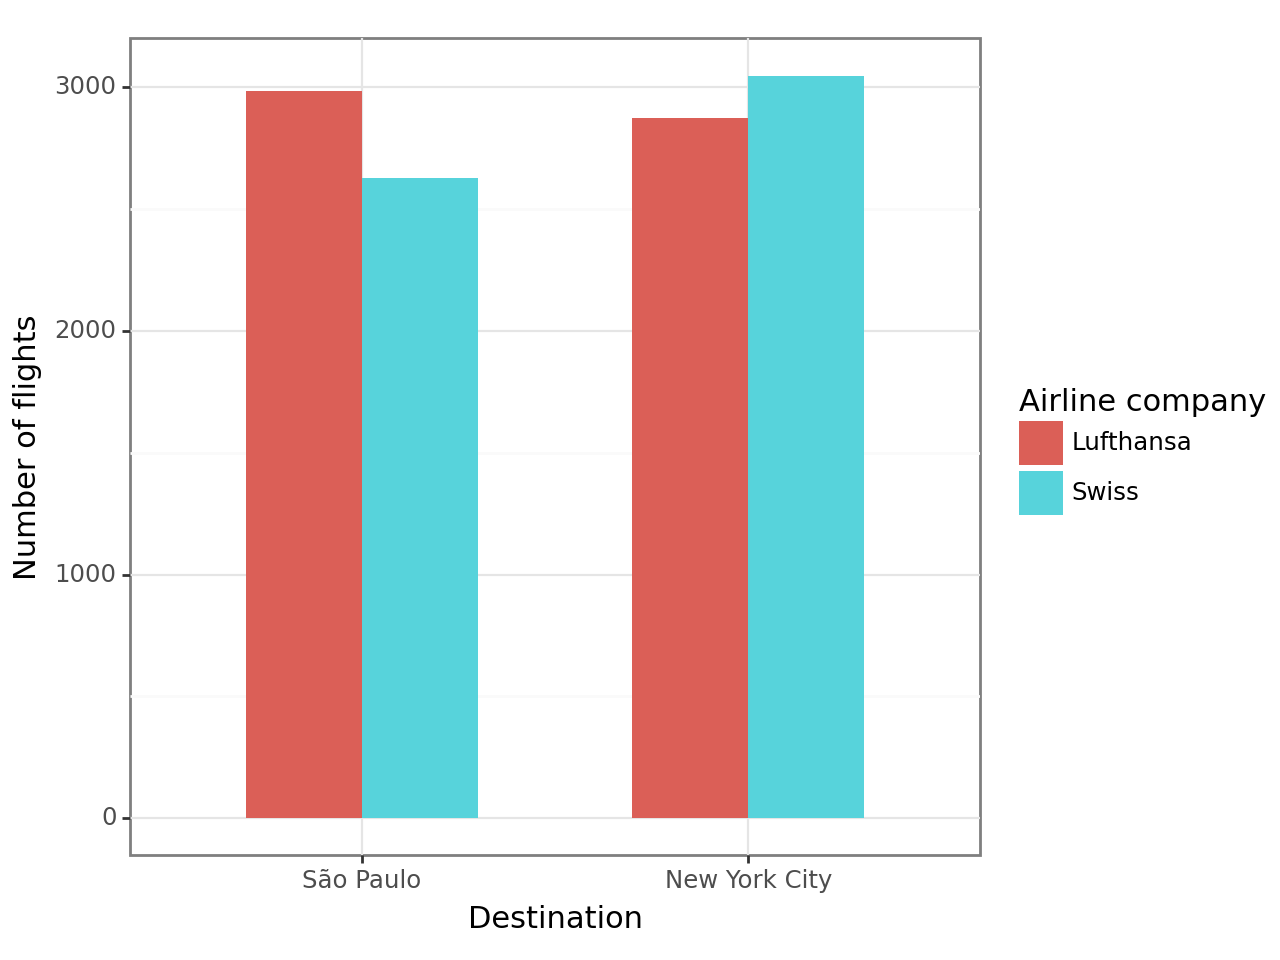
\includegraphics[width=0.7\textwidth]{images/1_dest_num_flights.png}
    \caption{Bar chart showing the number and frequency of flights to New York City and Sao Paulo operated by Lufthansa and Swiss Airline.}
    \label{fig:bar_pl}
\end{figure}

We also created additional stacked bar charts, shown in Figure~\ref{fig:stacked}, that display the minimum ticket price depending on the day of the week on which the flight is booked.
These charts allowed for easy visual comparison between the two companies for each destination.
We observed a clear variation in prices, mainly due to Swiss Airline, which tends to increase or decrease its prices more than Lufthansa.
For flights to New York City, shown in Figure~\ref{fig:stack_left}, booking on Monday, Tuesday, Saturday or Sunday would be more beneficial.
For flights to Sao Paulo, shown in Figure~\ref{fig:stack_right}, the price with Swiss Airline was significantly lower on Tuesday compared to other days of the week.
\begin{figure}
    \centering
    \subfigure[Stacked bar chart for flights to New York]{
      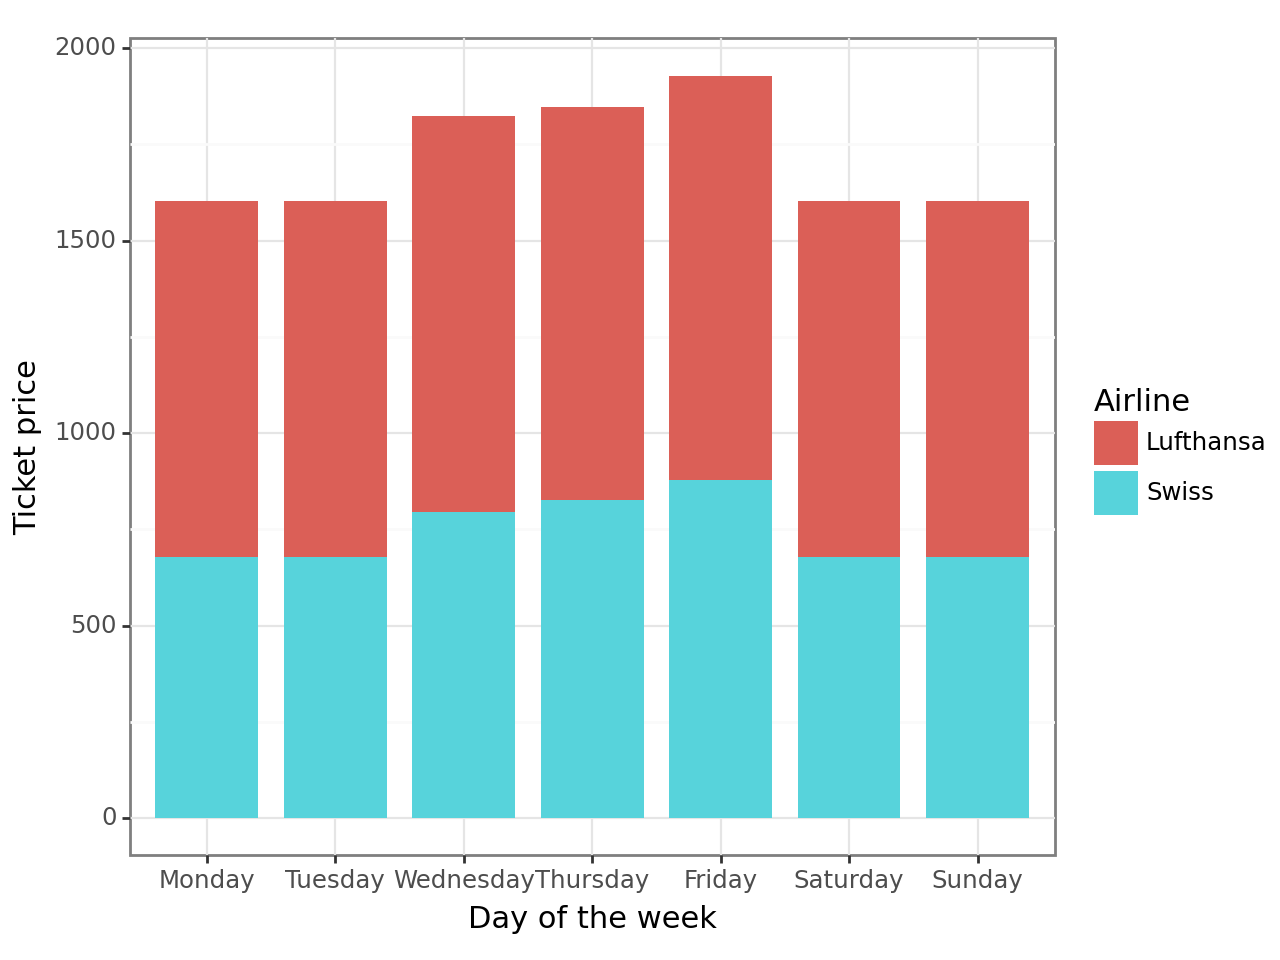
\includegraphics[width=0.45\textwidth]{images/2_1_day_ticket_price.png}
      \label{fig:stack_left}
    }
    \subfigure[Stacked bar chart for flights to Sao Paulo]{
      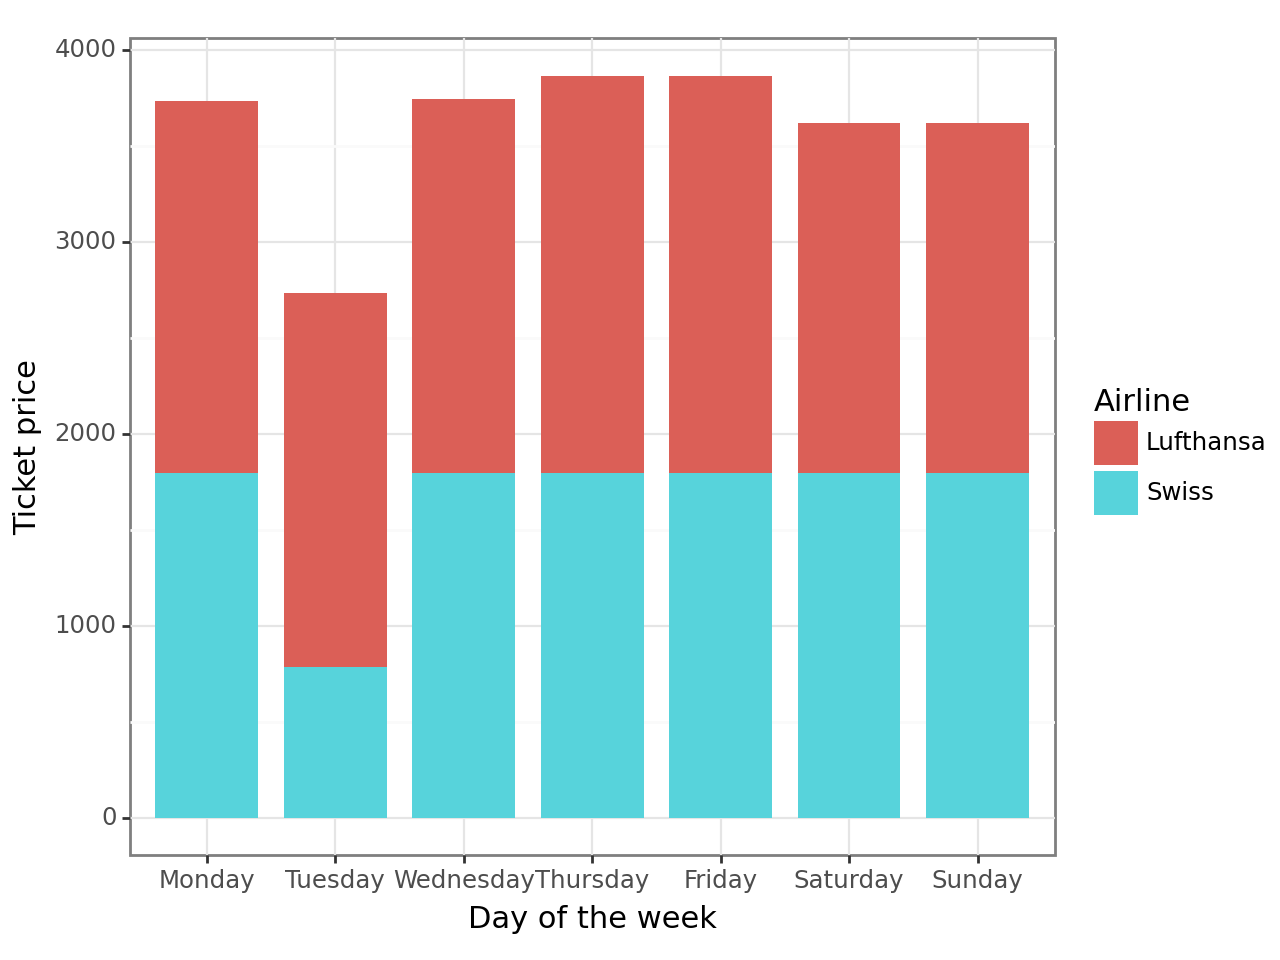
\includegraphics[width=0.45\textwidth]{images/2_2_day_ticket_price.png}
      \label{fig:stack_right}
    }
    \caption{Stacked bar charts showing the minimum ticket price for flights to New York City and Sao Paulo depending on the day of the week, operated by Lufthansa and Swiss Airline.}
    \label{fig:stacked}
\end{figure}

The second type of plot allows us to see the distribution of flight prices, shown by Figure~\ref{fig:box}.
These boxplots especially draw attention to outliers, representing prices that deviated from the typical price range of an airline.
The Figure~\ref{fig:box_left} reveals that, in the case of flights to New York City, there is a noticeable and higher variability in prices associated with Swiss Airline.
The opposite can be observed in the case of Sao Paulo, shown by Figure~\ref{fig:box_right}. Overall, prices are around 1000 Euros for New York City, but prices can go until 2000 Euros for Sao Paulo.
The mean shows that Swiss Airline offers lower prices specifically for each destination, in average.

\begin{figure}
    \centering
    \subfigure[Boxplot for flights to New York]{
      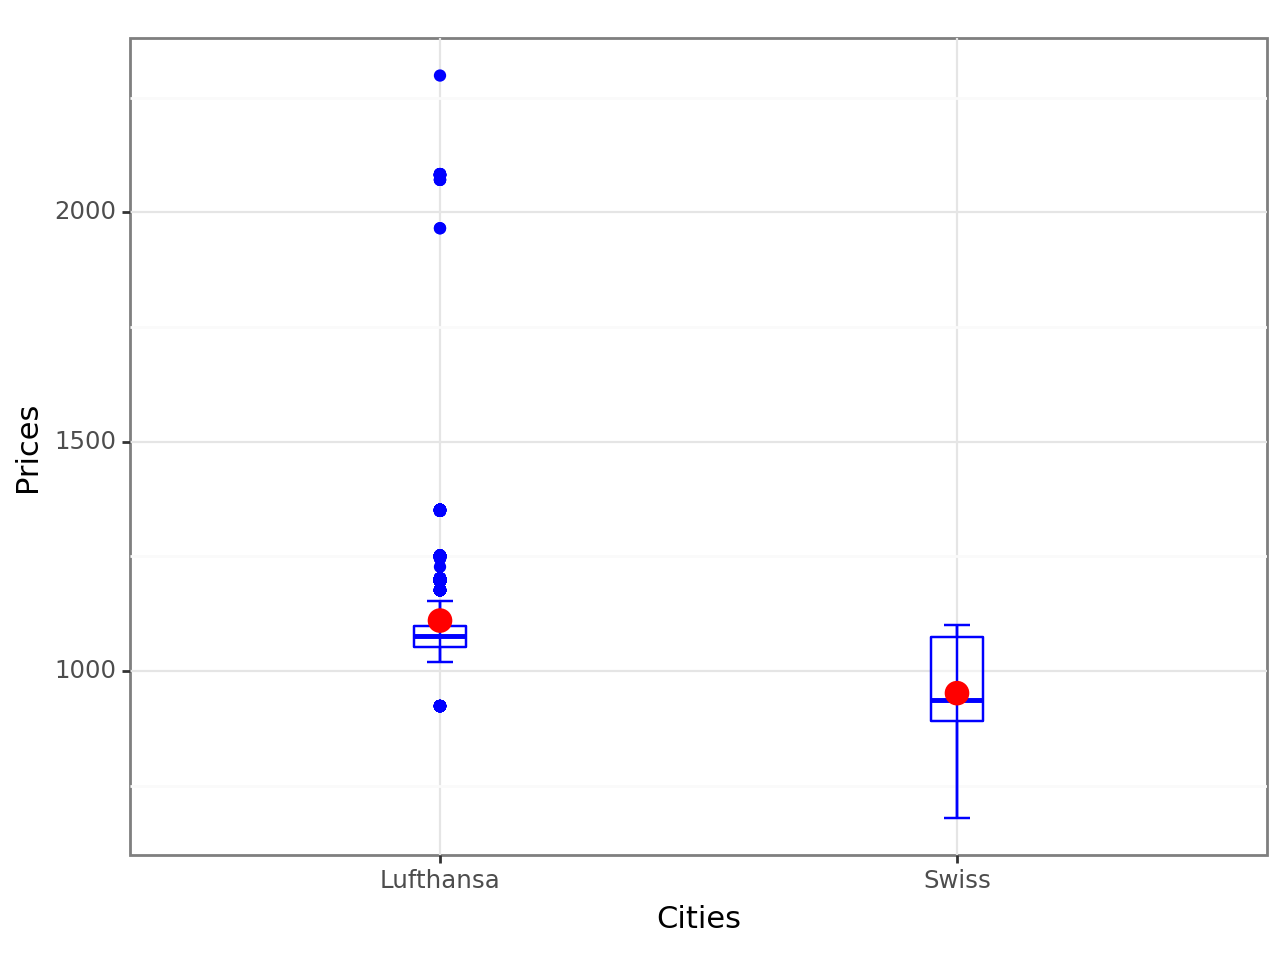
\includegraphics[width=0.45\textwidth]{images/3_1_cities_prices.png}
      \label{fig:box_left}
    }
    \subfigure[Boxplot for flights to Sao paulo]{
      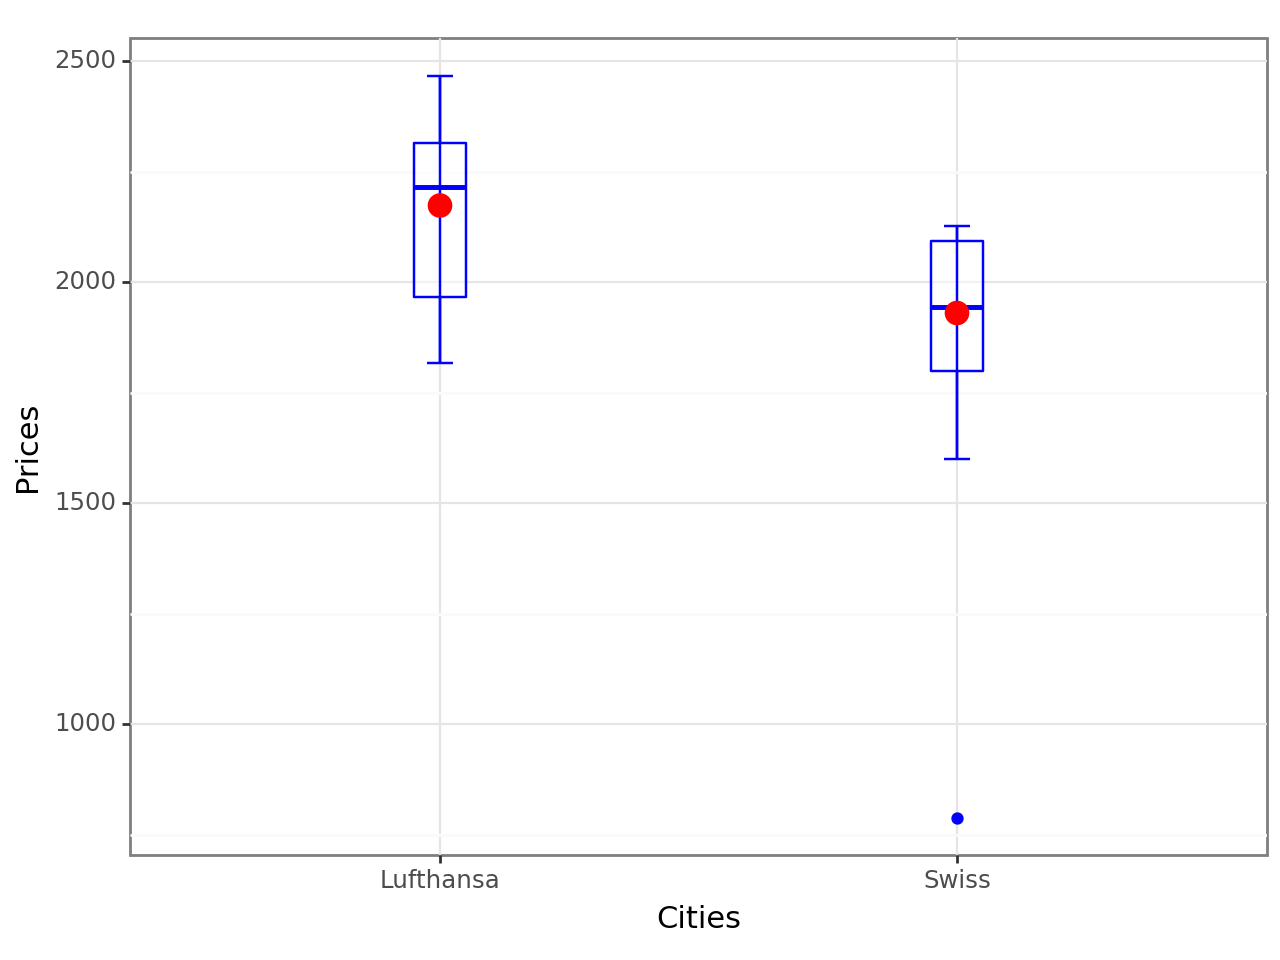
\includegraphics[width=0.45\textwidth]{images/3_2_cities_prices.png}
      \label{fig:box_right}
    }
    \caption{Flight price distribution for different airlines to New York City and Sao Paulo.}
    \label{fig:box}
\end{figure}

Line plots are essential for visualizing the fluctuations in prices over time, which allows for a better understanding of any patterns that may emerge.
As the departure date was approaching, as shown by Figure~\ref{fig:line_pl}, the average price of tickets for both destinations did begin to increase and varied more.
This highlights the importance of considering the timing of booking to secure more favorable prices.
Swiss Airline exhibits a rather consistent increase in prices for both New York City and Sao Paulo as the departure date approaches.
This suggests that booking earlier with Swiss Airline could result in more favorable prices.
On the other hand, Lufthansa's price trend is less obvious and does not show a clear pattern of increasing prices as the departure date approaches.
This could mean that booking timing may not be as crucial when flying with Lufthansa.

\begin{figure}
    \centering
    \subfigure[Flight price trend to NYC]{
      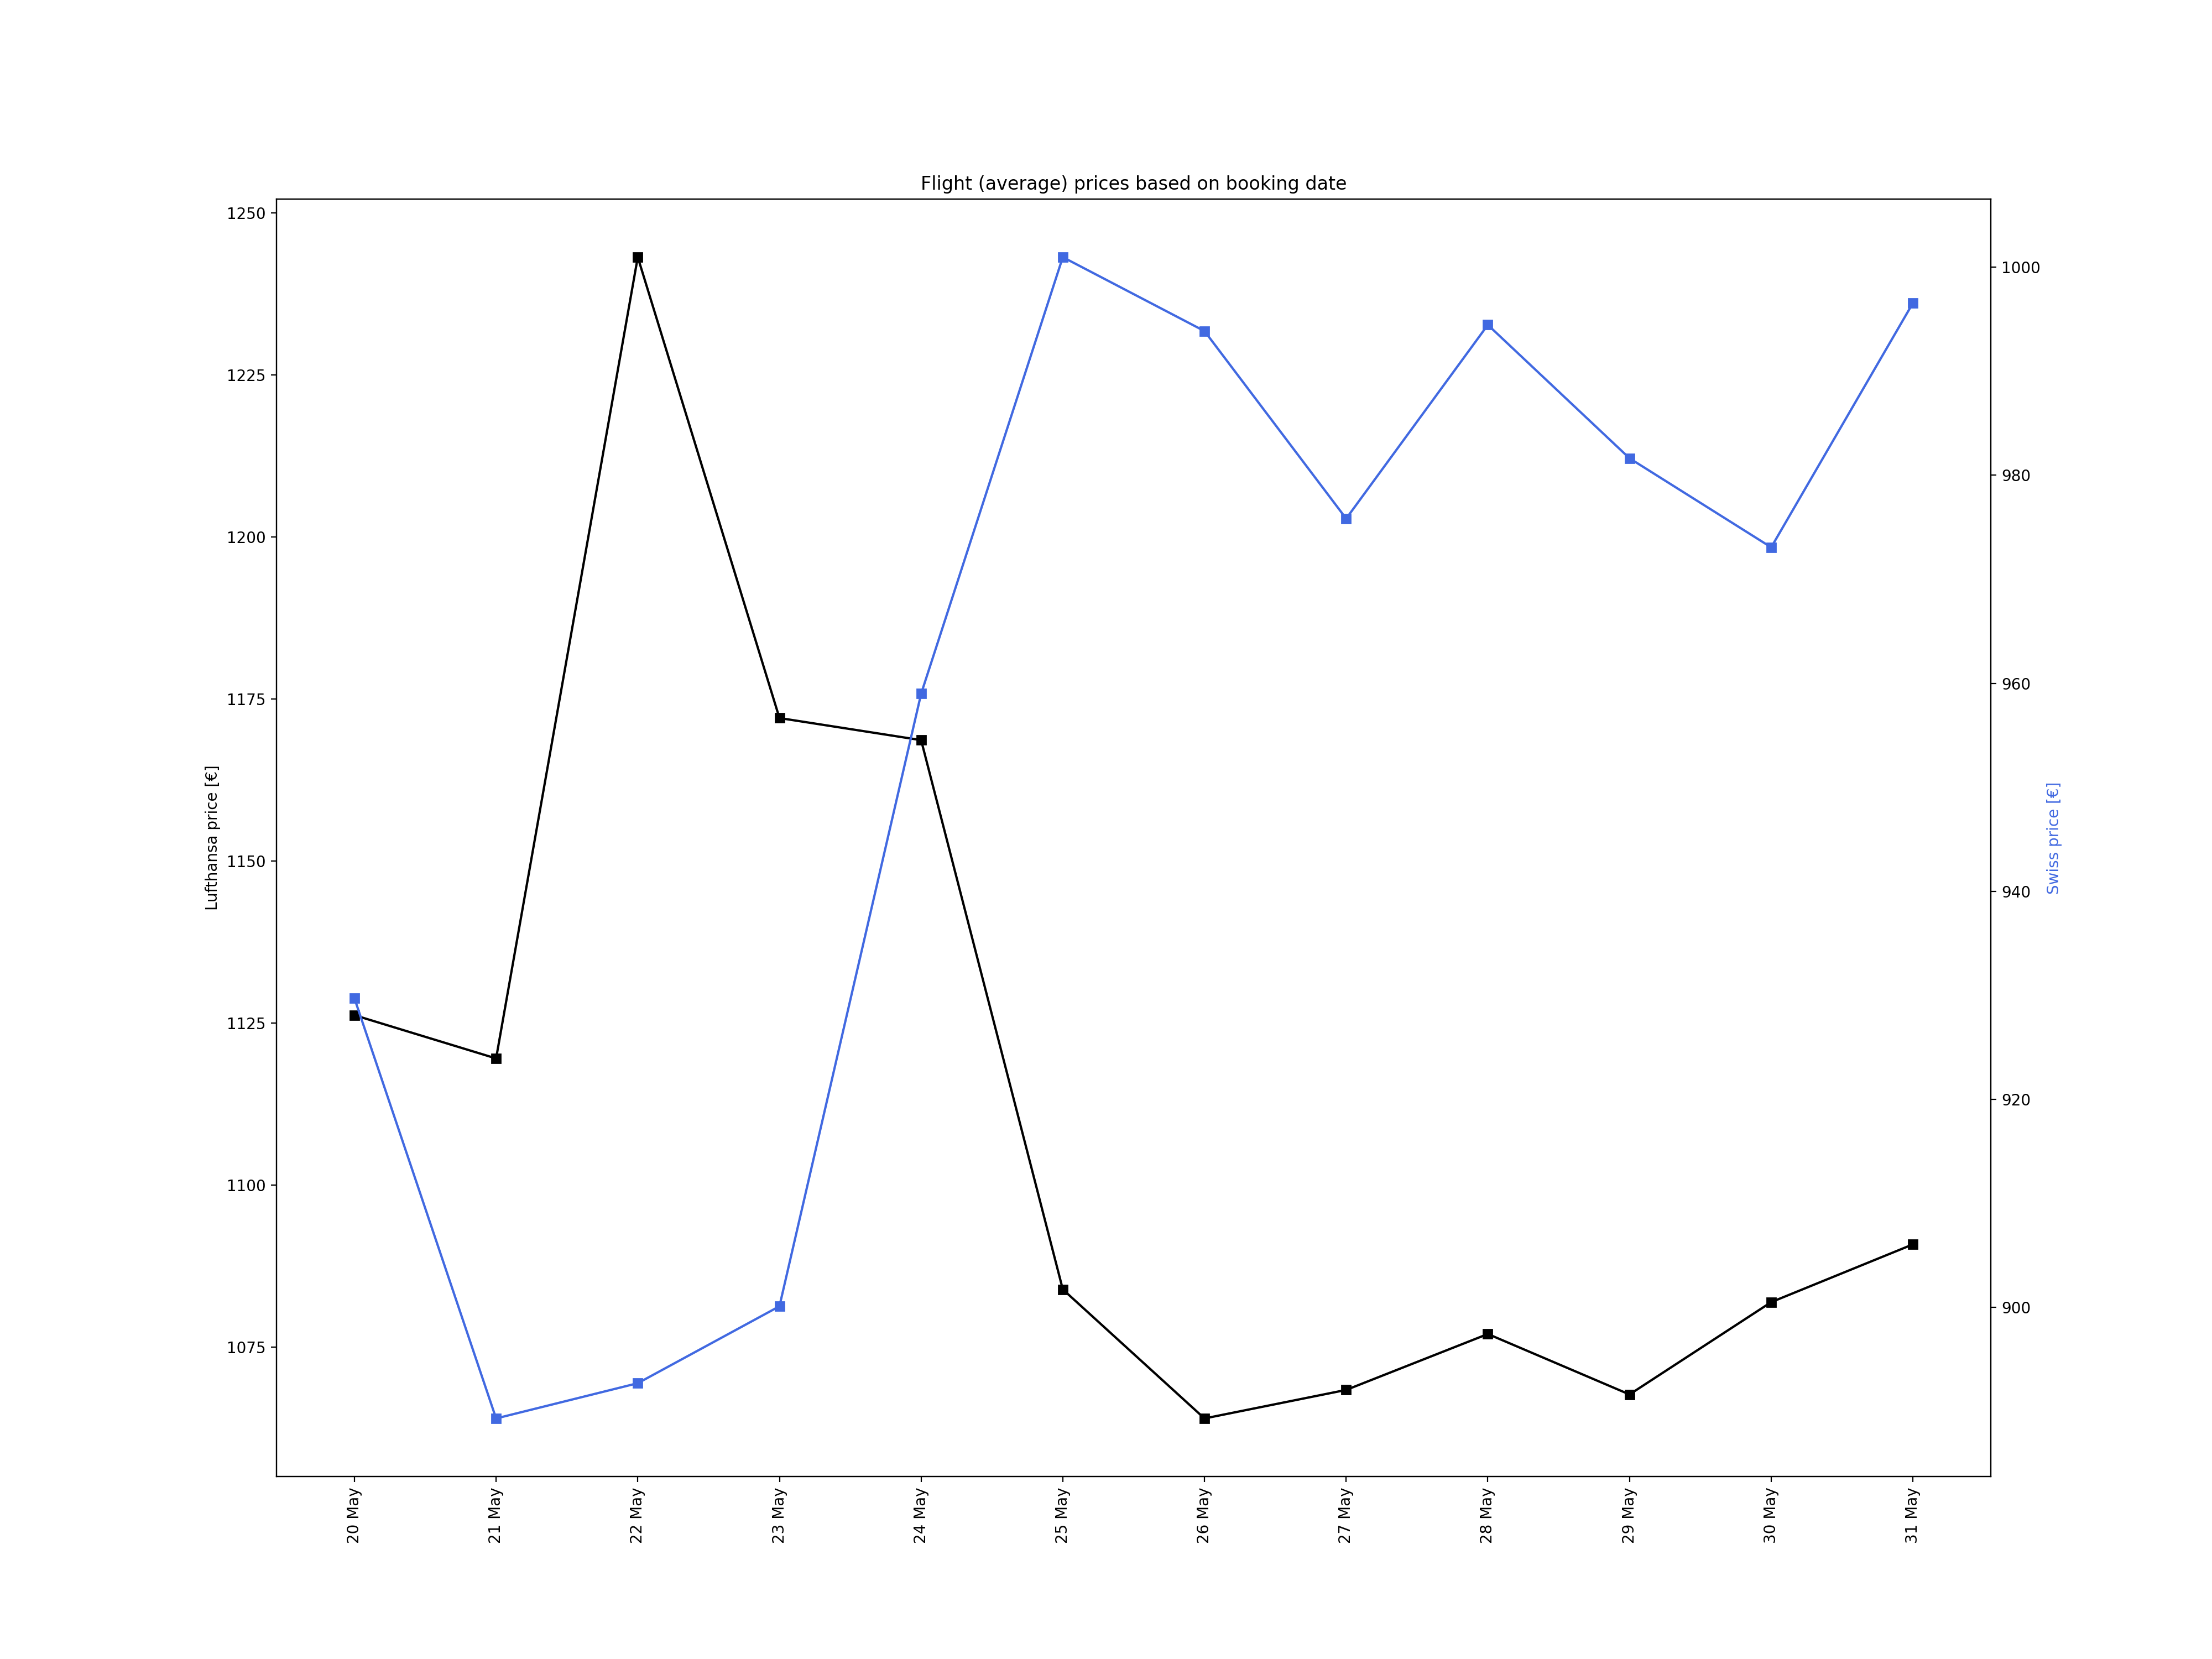
\includegraphics[width=0.45\textwidth]{images/4_1_hour_price_air.png}
      \label{fig:left}
    }
    \subfigure[Flight price trend to NYC]{
      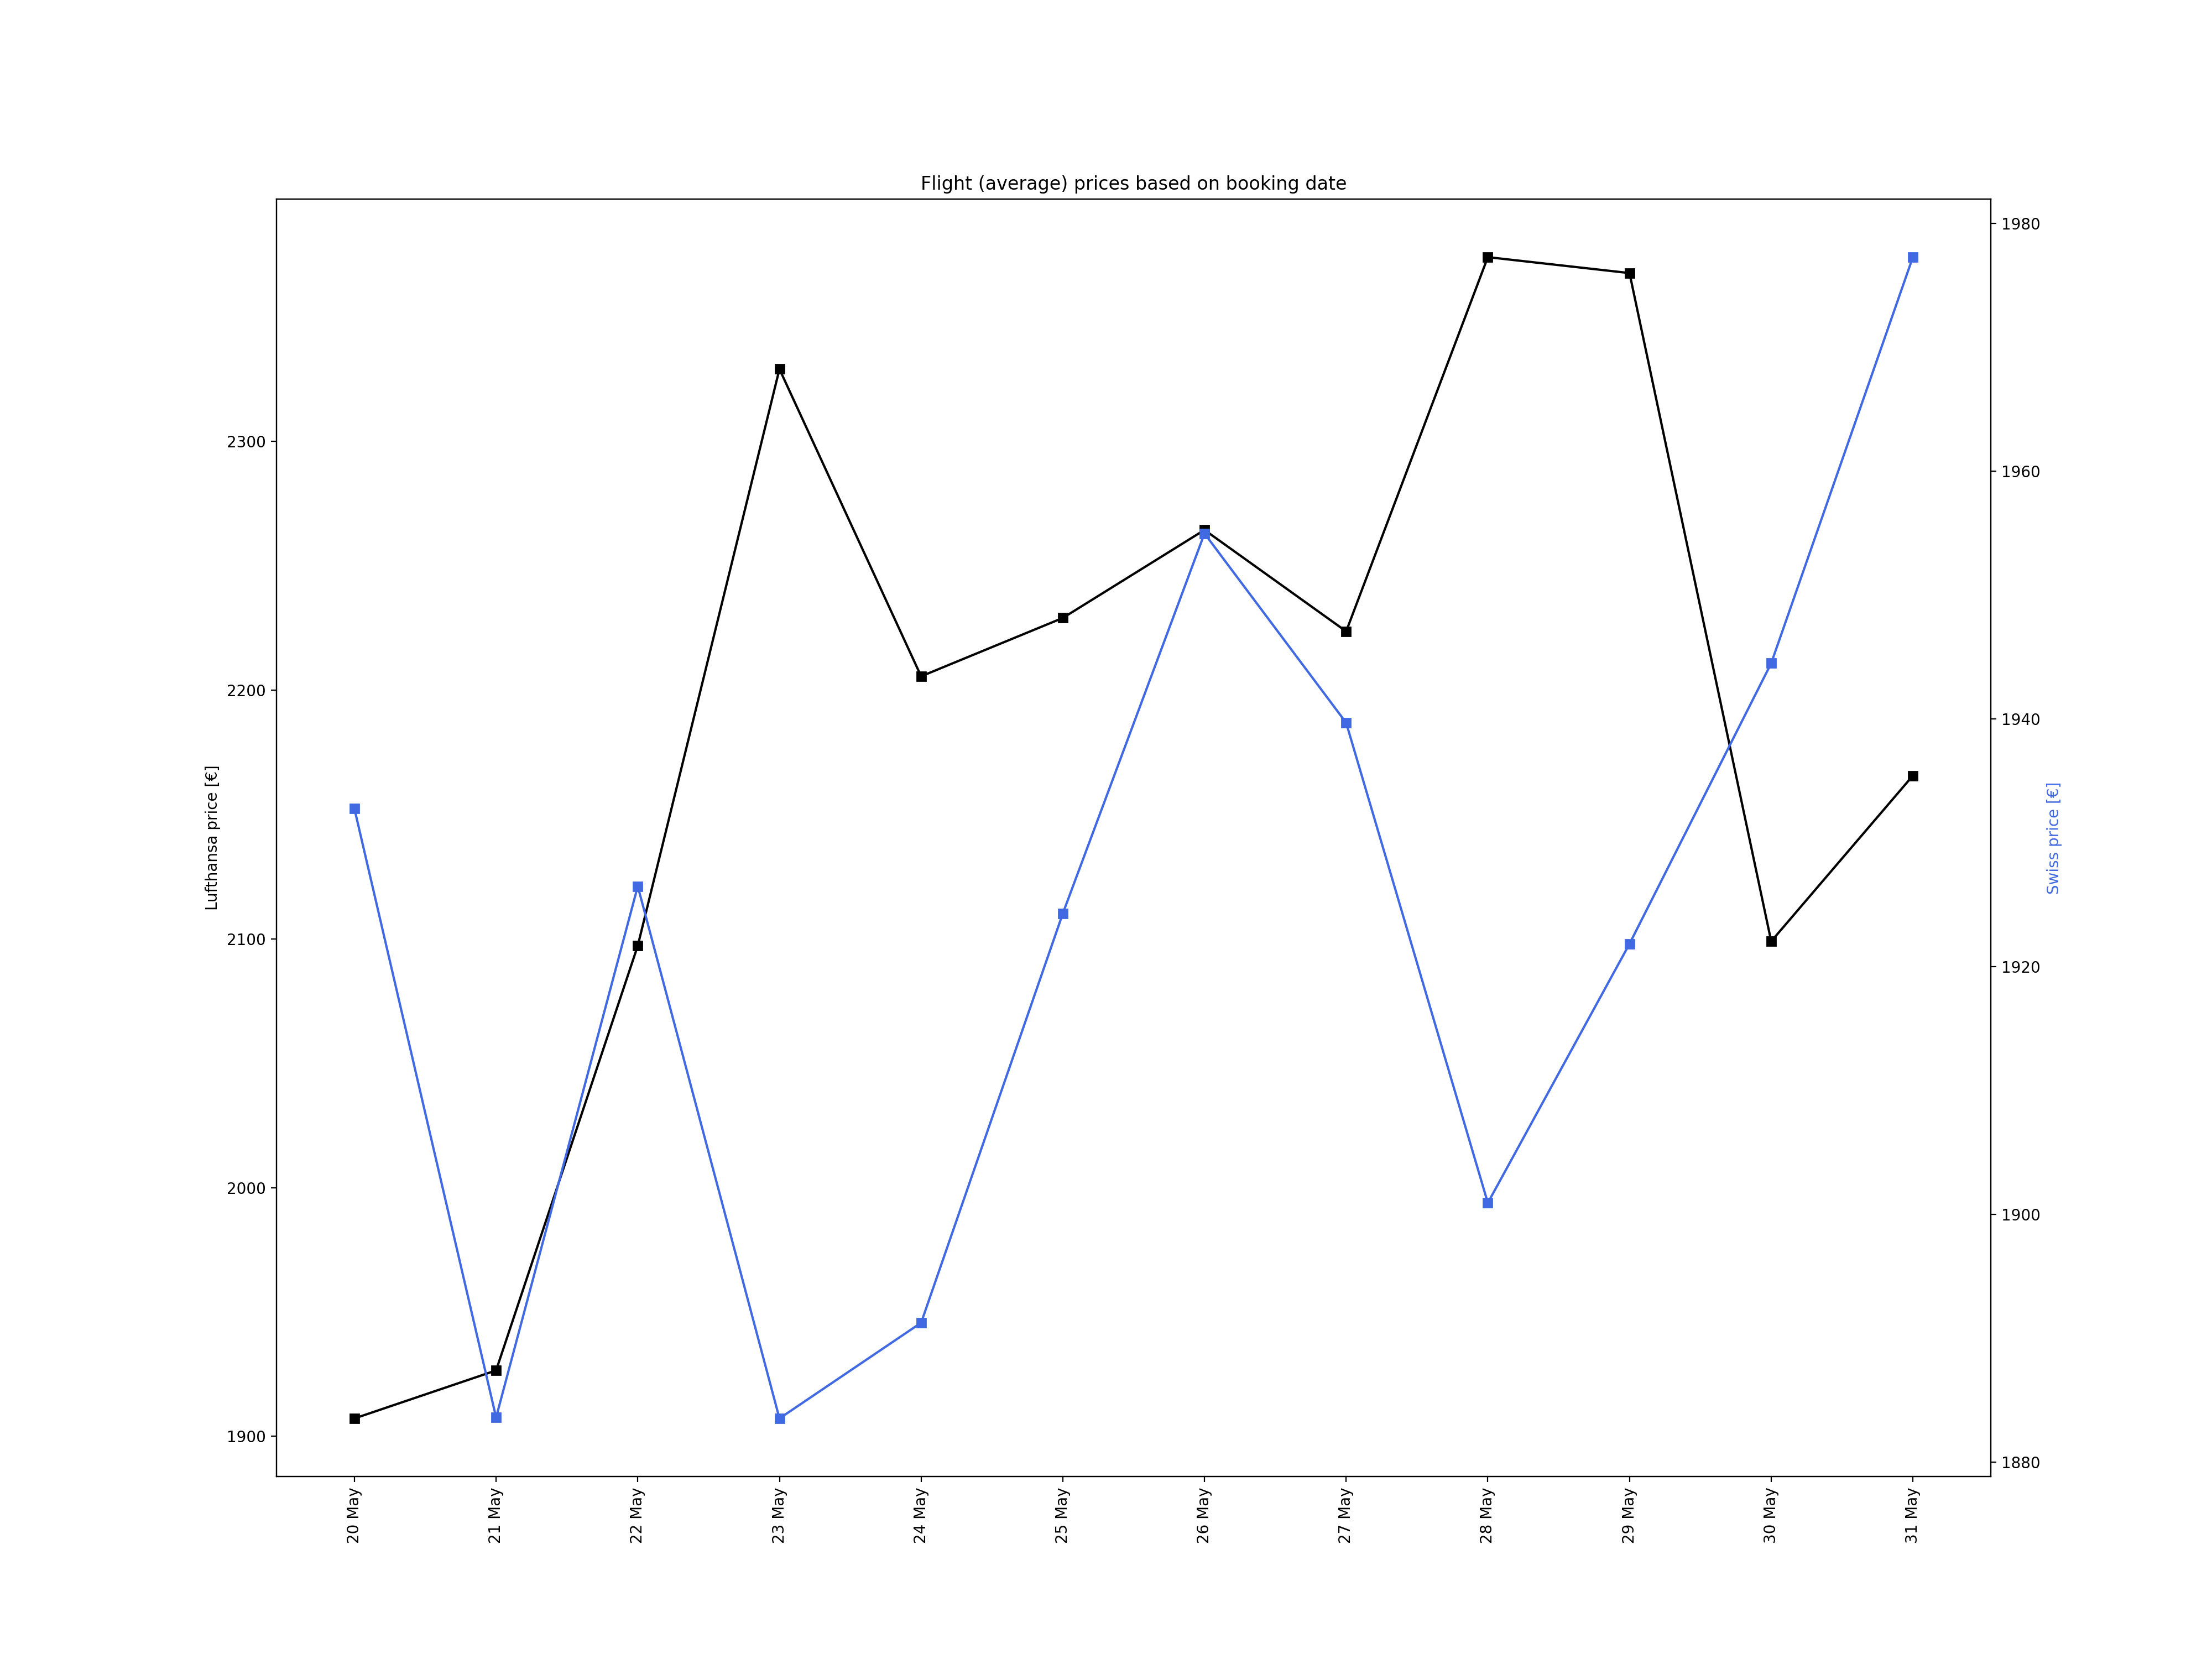
\includegraphics[width=0.45\textwidth]{images/4_2_hour_price_air.png}
      \label{fig:right}
    }
    \caption{Line plots showing the fluctuations in flight prices over time for Lufthansa and Swiss Airline to New York City and Sao Paulo.}
    \label{fig:line_pl}
\end{figure}

Scatter plots, Figure~\ref{fig:scatter}, are an effective way to visualize the relationship between flight cost and duration.
By visually assessing the correlation between these two variables, we were able to gain insights into their relationship.
For example, the Figure~\ref{fig:scat_left} for New York City revealed a clear negative correlation between flight price and duration, indicating that longer flights tend to be less expensive.
This could be a useful feature for predicting flight prices. In contrast, the relationship between these variables was less clear for Sao Paulo, but still tended towards a negative correlation, as shown by Figure~\ref{fig:scat_right}.
Additionally, we observed that Lufthansa flights tended to have higher costs for the same flight duration.
\begin{figure}
    \centering
    \subfigure[Scatter plot for flights New York]{
      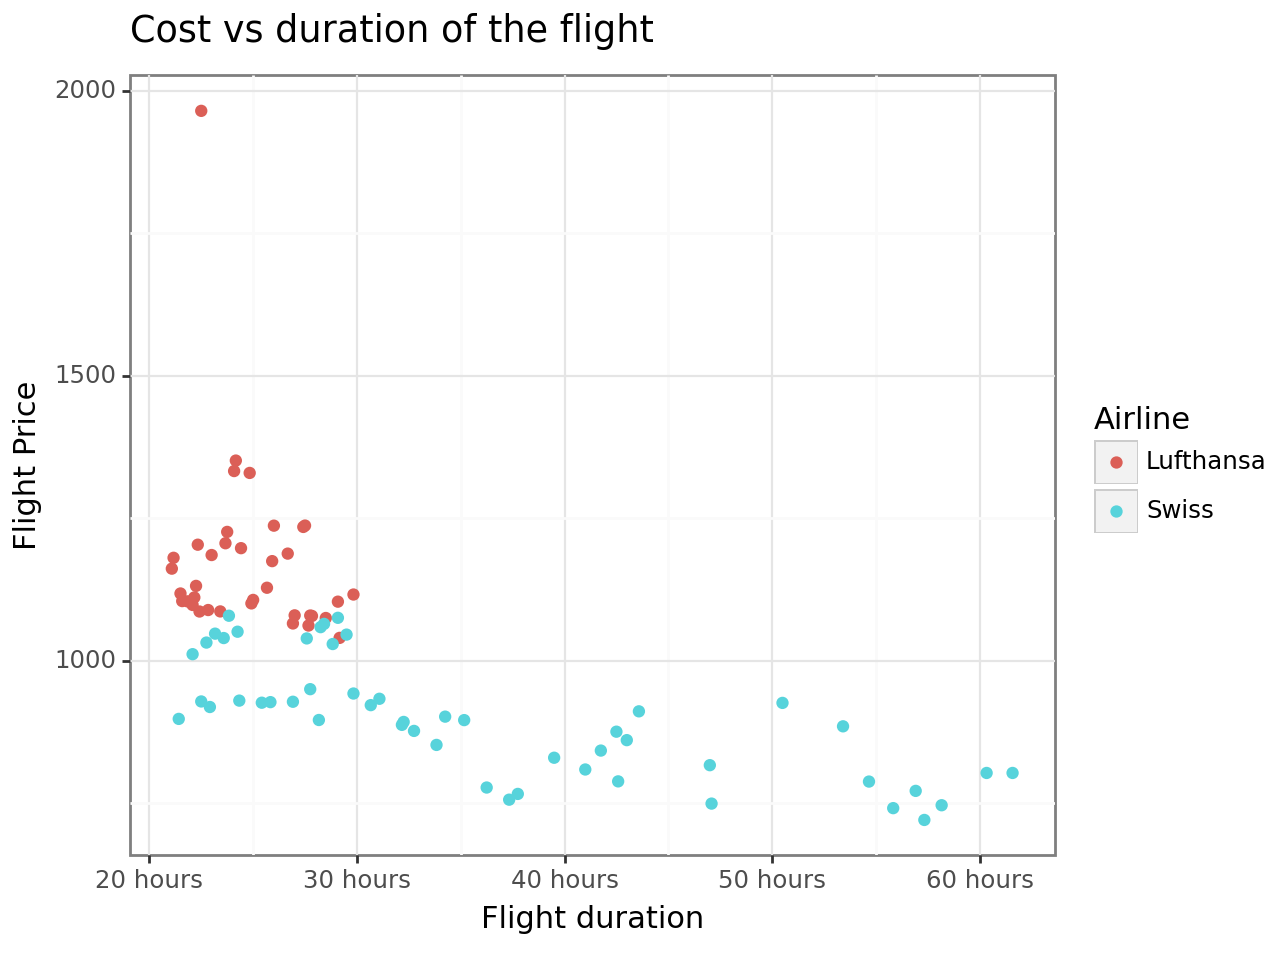
\includegraphics[width=0.45\textwidth]{images/5_1_price_duration.png}
      \label{fig:scat_left}
    }
    \subfigure[Scatter plot for flights Sao Paulo]{
      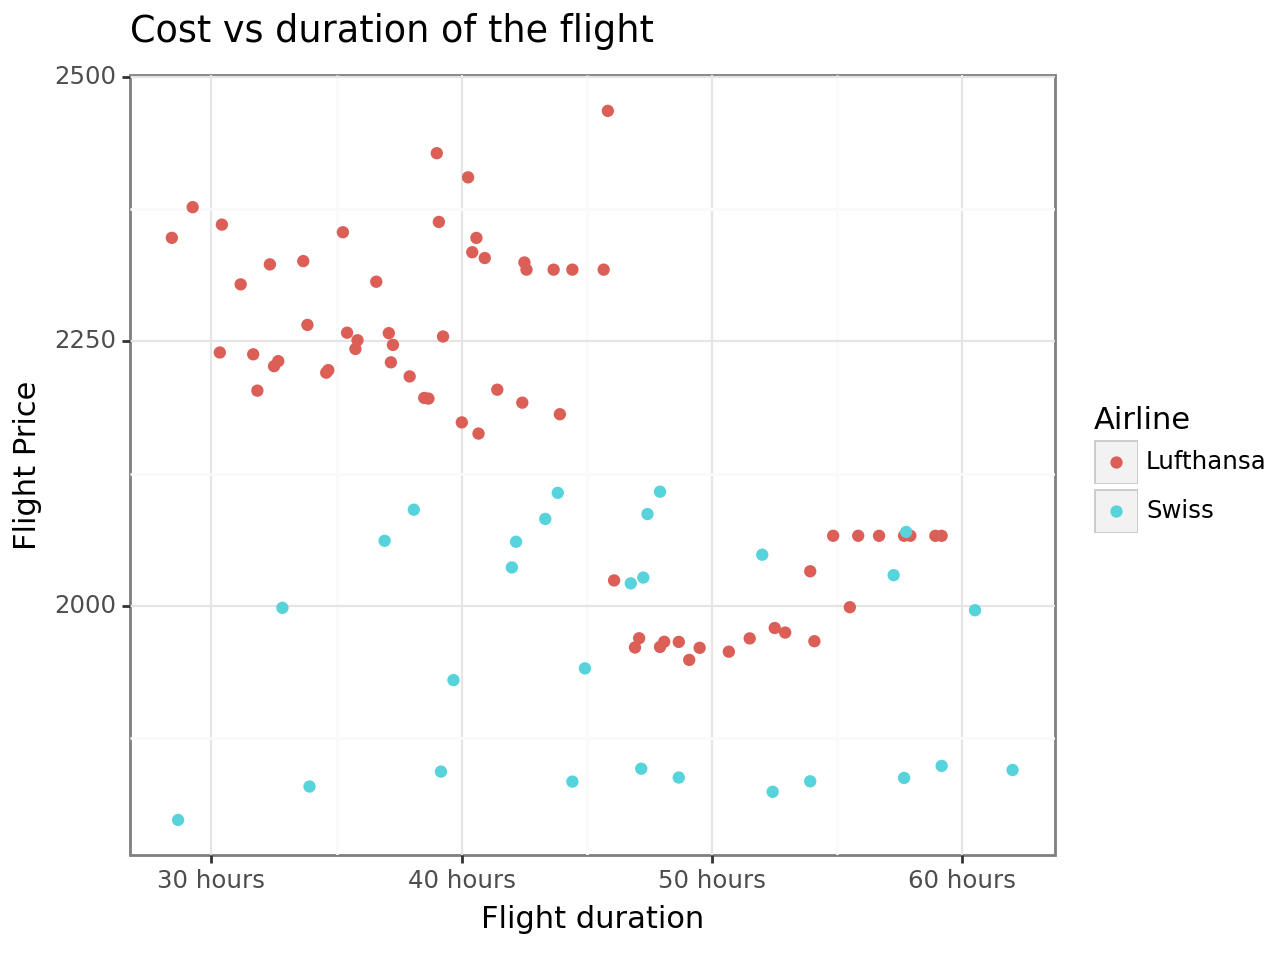
\includegraphics[width=0.45\textwidth]{images/5_2_price_duration.png}
      \label{fig:scat_right}
    }
    \caption{Scatter plots showing the relationship between flight cost and duration for New York City and Sao Paulo.}
    \label{fig:scatter}
\end{figure}

The final step in our data visualization process was to create a heatmap of all numerical variables to better identify features for use in data modeling.
Our analysis of the New York City destination revealed a strong negative correlation between ticket price and flight duration, as previously indicated by the scatter plot.
Additionally, departure time also appeared to be negatively correlated with our prediction target.
For Sao Paulo, prices showed a stronger correlation with flight duration and time-related variables.
These observations and anlysis concerning the heatmaps is illustrated by Figure~\ref{fig:heat}.
\begin{figure}
    \centering
    \subfigure[Heatmap for flights to New York]{
      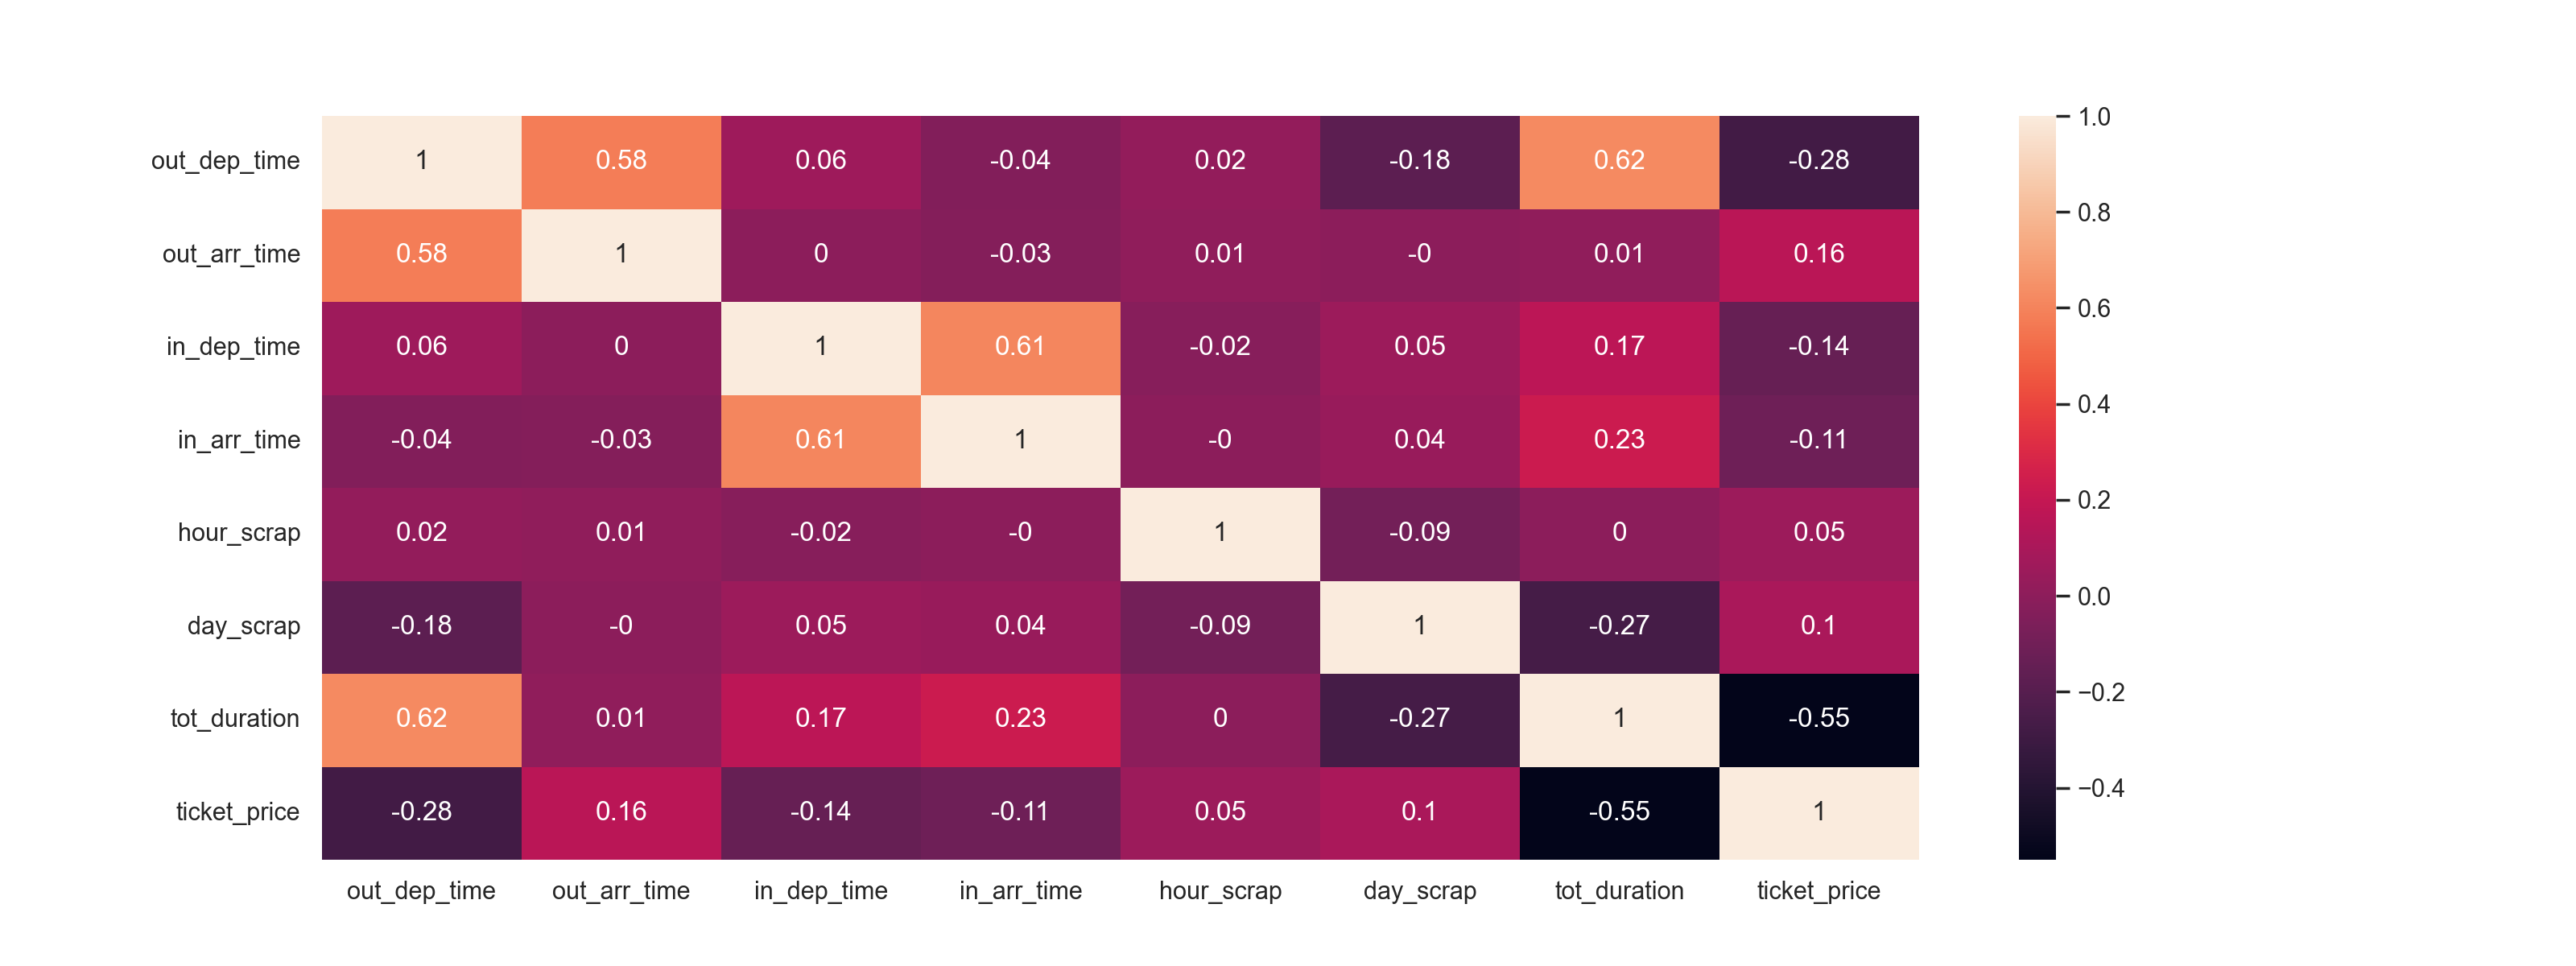
\includegraphics[width=1\textwidth]{images/6_1_heatmap.png}
      \label{fig:left_heat}
    }
    \subfigure[Heatmap for flights for Sao paulo]{
      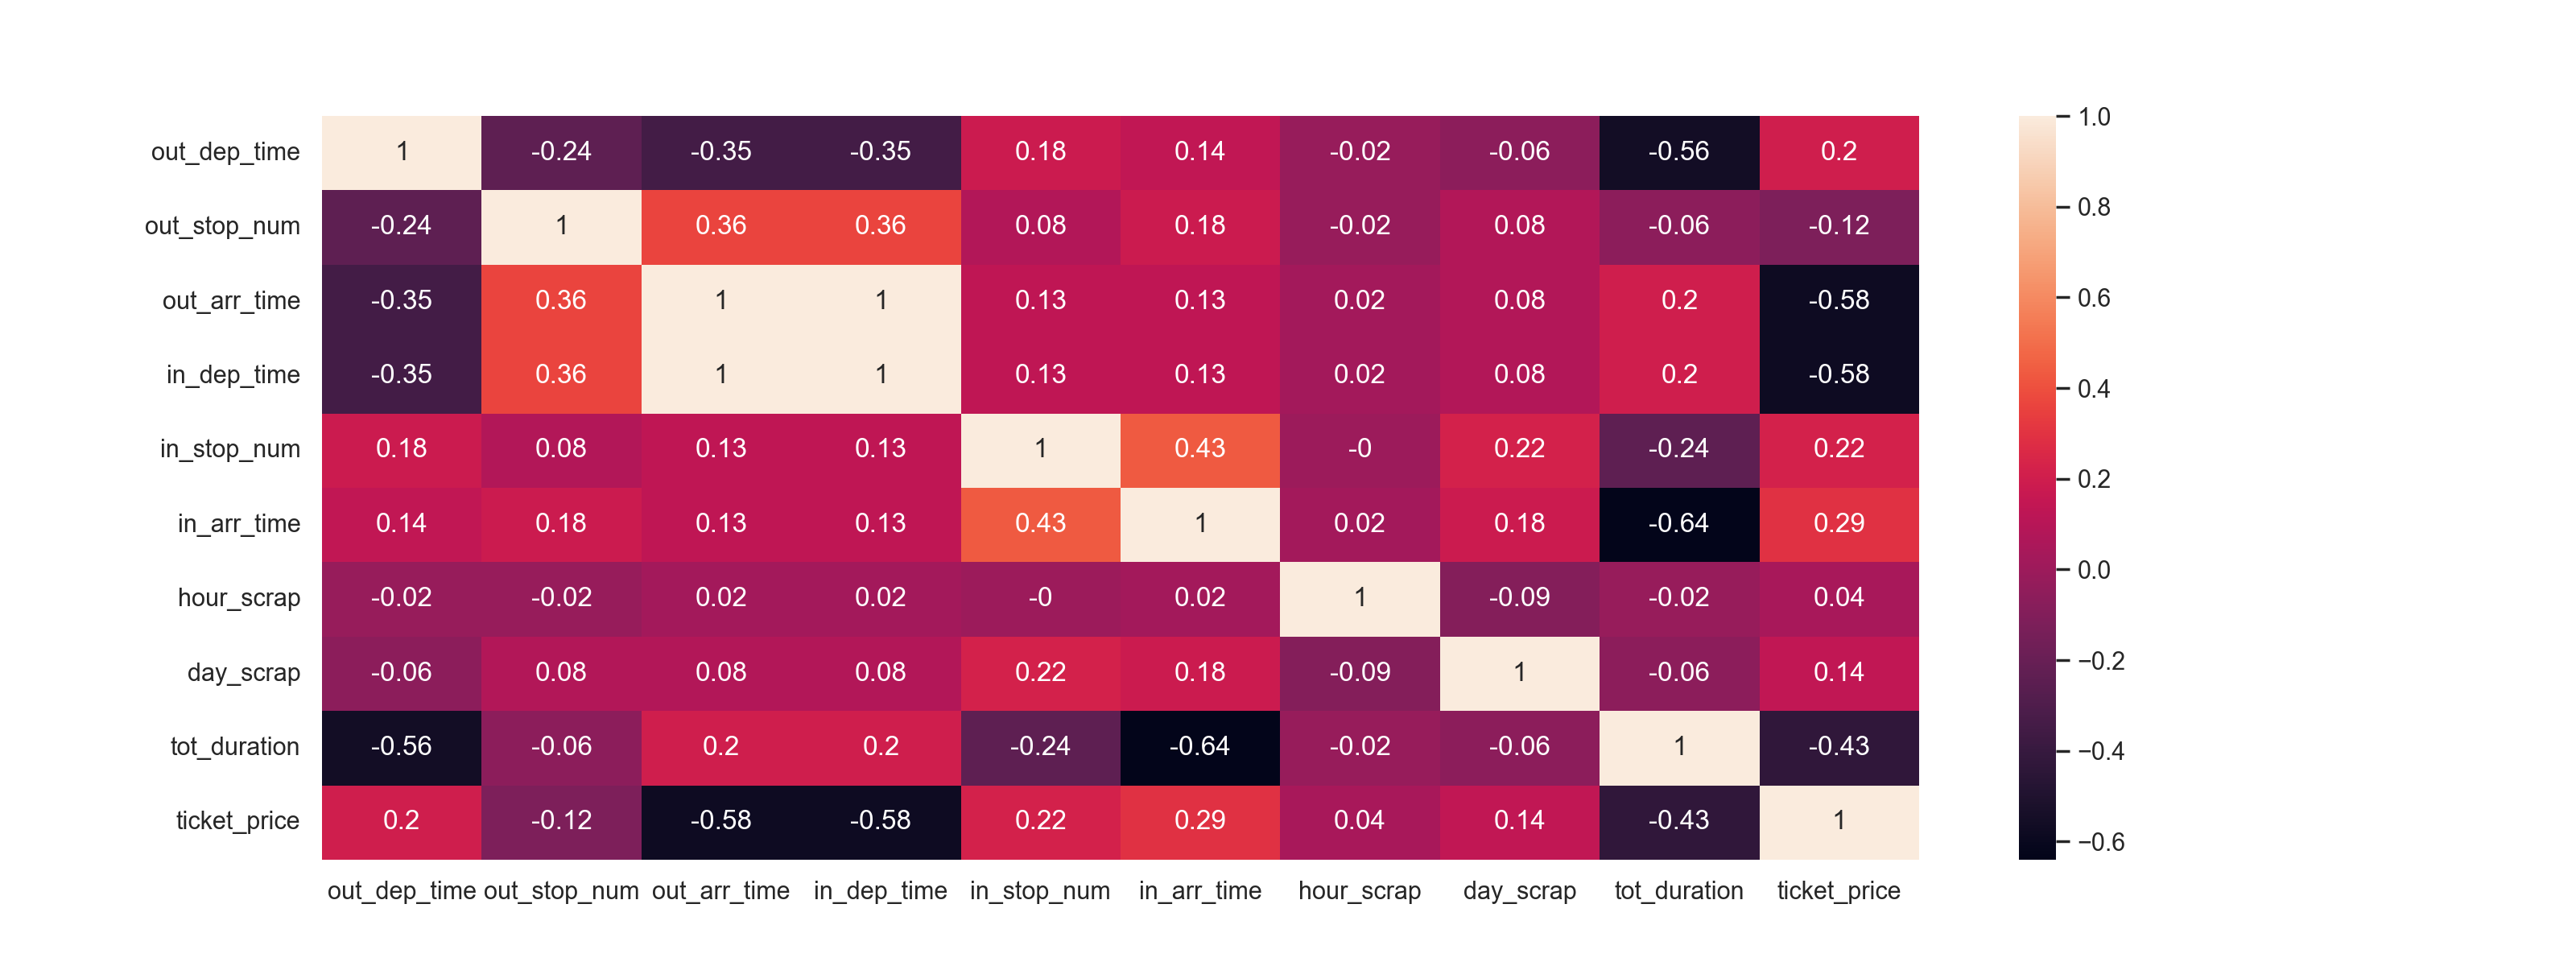
\includegraphics[width=1\textwidth]{images/6_2_heatmap.png}
      \label{fig:right_heat}
    }
    \caption{Heatmaps showing correlations between numerical variables for New York City and Sao Paulo.}
    \label{fig:heat}
\end{figure}

% \begin{figure}
%     \centering
%     \subfigure[Left figure]{
%       \includegraphics[width=0.45\textwidth]{images/}
%       \label{fig:left}
%     }
%     \subfigure[Right figure]{
%       \includegraphics[width=0.45\textwidth]{images/}
%       \label{fig:right}
%     }
%     \caption{Combined figure}
%     \label{fig:combined}
% \end{figure}



\subsection{Data modelling}
\label{sec:data}
The data visualization process has yielded several key insights that could inform data modeling efforts. 
For instance, line plots have shown that ticket prices for both New York City and Sao Paulo tend to increase and exhibit greater variation as the departure date approaches.
In particular, Swiss Airline has displayed a consistent increase in prices. Scatter plots have also revealed a distinct negative correlation between flight price and duration for New York City.
While the relationship for Sao Paulo is less clear, it still tends towards a negative correlation. Heatmaps have further shown strong negative correlations between ticket price and flight duration for New York City, as well as stronger correlations between prices and flight duration/time-related variables for Sao Paulo. 
These insights highlight the importance of considering factors such as booking timing, flight duration, and time-related variables when modeling data.

In this project, several libraries and functions from the scikit-learn and statsmodels packages were utilized to perform data analysis and modeling. 
The data was split into training and testing sets using the train\_test\_split function, while cross-validation was performed using the cross\_val\_score function.
The performance of the models was evaluated using various metrics, including accuracy\_score, mean\_absolute\_error, mean\_squared\_error, and r2\_score.
Although several regression models were employed to fit the data and make predictions, including LinearRegression, LogisticRegression and LogisticRegressionCV,
only the results from the LinearRegression model will be taken into account.
Additionally, statistical analysis was performed and multicollinearity was assessed using the statsmodels library and its api module as well as the variance\_inflation\_factor function.

Several models were tested on different dataframes. Ultimately, a linear regression model was selected with the following function: 
\\
$Ticket\_price = \beta_0 + \beta_1 \times tot\_duration\_seconds + \beta_2 \times hour\_scrap + \beta_3 \times airline\_company\_dummy + \beta_4 \times destination\_dummy + \beta_5 \times out\_dep\_time\_dummy + \beta_6 \times in\_arr\_time\_dummy + \beta_7 \times day\_of\_week\_\*$.

The linear regression model incorporates several independent variables and a dependent variable.
The dependent variable is ticket\_price, which represents the ticket price for a flight and can take any non-negative numerical value.
The first independent variable is tot\_duration\_seconds, which denotes the total duration of the flight in seconds.
The second variable is hour\_scrap, which specifies the hour at which the data was collected.
The third and fourth variables, airline\_company\_dummy and destination\_dummy, are dummy variables that represent the airline company and destination, respectively.
The fifth and sixth variables, out\_dep\_time\_dummy and in\_arr\_time\_dummy, are dummy variables that indicate the departure time from the origin and arrival time at the destination, respectively.
Lastly, day\_of\_week\_* represents dummy variables that indicate the day of the week on which the data was collected.

\begin{table}[H]
  \centering
  \begin{tabular}{l c}
  \hline
   & \textbf{Values} \\
  \hline
  \textbf{Intercept} & 2097.4909712064773 \\
  \textbf{Training RMSE} & 522.364425 \\
  \textbf{Test RMSE} & 524.069444 \\
  \textbf{Cross-validation RMSE} & 516.31323 \\
  \textbf{Mean Absolute Error} & 171.879278 \\
  \textbf{Mean Squared Error} & 274648.782087 \\
  \textbf{Root Mean Squared Error} & 524.069444 \\
  \textbf{R-squared} & 0.552468 \\
  \hline
  \end{tabular}
  \caption{Different metrics to assess the model and their results}
  \label{tab:my_tab}
\end{table}

The linear regression model was assessed and several values were obtained, as shown by Table~\ref{tab:my_tab}. 
The intercept value of 2097.49 represents the expected value of the dependent variable \(ticket\_price\) when all independent variables are equal to zero.
The training and test RMSE values of 522.36 and 524.07, respectively, represent the root mean squared error of the model on the training and test data.
The cross-validation RMSE value of 516.31 represents the root mean squared error of the model when evaluated using cross-validation.
The mean absolute error value of 171.88 represents the average absolute difference between the predicted and actual values of the dependent variable.
The mean squared error value of 274648.78 represents the average squared difference between the predicted and actual values of the dependent variable.
The root mean squared error value of 524.07 represents the square root of the mean squared error. 
The R-squared value of 0.55 represents the proportion of variance in the dependent variable that is explained by the independent variables in the model.

\begin{table}[H]
  \centering
  \begin{tabular}{l c c}
  \hline
   & \textbf{coef} & \textbf{p-values} \\
  \hline
  \textbf{const} & 2103.6217 & 1.613956e-219 \\
  \textbf{tot\_duration\_seconds} & -0.0011 & 5.714598e-08 \\
  \textbf{hour\_scrap} & -2.8844 & 5.003298e-02 \\
  \textbf{day\_scrap} & 16.5914 & 2e-24\\
  \textbf{airline\_company\_dummy}&-291&2e-128\\
  \textbf{destination\_dummy}&-1207&0\\
  \textbf{out\_dep\_time\_dummy}&-159&1e-33\\
  \textbf{in\_arr\_time\_dummy}&89&2e-09\\
  \hline
  \end{tabular}
  \caption{Coefficients of the model and their p-values}
  \label{tab:my_tab1}
\end{table}

The coefficients and p-values for each independent variable represent the estimated effect of that variable on the dependent variable and the statistical significance of that effect, respectively.
For example, the coefficient for tot\_duration\_seconds is -0.0012, indicating that for every one-unit increase in tot\_duration\_seconds, ticket\_price is expected to decrease by 0.0012 units on average, holding all other variables constant.
The p-value for tot\_duration\_seconds is 5.71e-08, indicating that this effect is statistically significant at a conventional level \(e.g., p < 0.05\). 
Similarly, the coefficient for hour\_scrap is -2.31, indicating that for every one-unit increase in hour\_scrap,
ticket\_price is expected to decrease by 2.31 units on average, holding all other variables constant. 
The p-value for hour\_scrap is 0.050, indicating that this effect is marginally statistically significant at a conventional level.
They are summarize by the Table~\ref{tab:my_tab1}.

Furthermore, the variance inflation factor (VIF) was calculated for each independent variable in the linear regression model.
The VIF is a measure of the degree to which the variance of the estimated regression coefficients is inflated due to multicollinearity among the independent variables.
A VIF value greater than 5 or 10 is often considered to indicate high multicollinearity. In this case, the VIF values for all independent variables were below 5, indicating that multicollinearity is not a major concern in this model. 
The VIF values can be found in the Table~\ref{tab:vif}.
\begin{table}[H]
  \centering
  \begin{tabular}{l c}
  \hline
  \textbf{feature} & \textbf{VIF} \\
  \hline
  const & 142.799773 \\
  tot\_duration\_seconds & 2.393894 \\
  hour\_scrap & 1.008921 \\
  day\_scrap & 1.054136 \\
  airline\_company\_dummy & 1.175422 \\
  destination\_dummy & 2.411166 \\
  out\_dep\_time\_dummy & 1.460508 \\
  in\_arr\_time\_dummy & 1.249996 \\
  \hline
  \end{tabular}
  \caption{VIF values for each feature}
  \label{tab:vif}
\end{table}

In conclusion, the linear regression model was chosen for several reasons.
First, the model incorporates several relevant independent variables, including tot\_duration
\_seconds, hour\_scrap, airline\_company\_dummy, destination\_dummy, out\_dep\_time\_dummy, and in\_arr\_time\_dummy.
These variables were found to have statistically significant effects on the dependent variable (ticket\_price) based on their p-values.
Second, the model was assessed using various metrics and was found to have a reasonable level of predictive accuracy. 
For instance, the R-squared value of 0.55 indicates that the model explains a moderate proportion of variance in the dependent variable.
Third, the variance inflation factor (VIF) values for all independent variables were below 5, indicating that multicollinearity is not a major concern in this model.
Overall, these factors suggest that this linear regression model is a suitable choice for modeling the relationship between the independent variables and ticket\_price.

By using this model, ticket prices were predicted for different combinations of day and hour when data was collected.
The predicted ticket prices are summarized in the Table~\ref{tab:pred}.
For example, for data collected on a Monday at 8:00 AM for a flight from New York to Lufthansa, the predicted ticket price is 1237.32.
For data collected on a Sunday at 22:00 PM for a flight from Sao Paulo to Swiss, the predicted ticket price is 2136.93.
These predictions can provide useful information for individuals looking to book flights and can help them make informed decisions about when to book their tickets.

\begin{table}[h!]
  \centering
  \begin{tabular}{l l l l l l l l l l l}
  & & Day & Monday & Tuesday & Wednesday & Thursday & Friday & Saturday & Sunday \\
  Destination & Airline & Hour & & & & & & & \\
  New York & Lufthansa & 8 & 1237.32 & 1269.55 & 1385.51 & 1227.89 & 1220.52 & 1208.47 & 1205.67 \\
  & & 10 & 1231.43 & 1263.65 & 1379.61 & 1221.99 & 1214.62 & 1202.58 & 1199.78\\
  & & 12 & 1225.53 & 1257.75 & 1373.71 & 1216.10 & 1208.73 &  1196.68 & 1193.88\\
  & & 14 & 1219.63 & 1251.86 & 1367.81 & 1210.20 & 1202.83 & 1193.88 & 1187.98\\
  & & 16 & 1213.73 & 1245.96 & 1361.92 & 1204.30 & 1196.93 & 1184.88 & 1182.09 \\
  & & 18 & 1207.84 & 1240.06 & 1356.02 & 1198.41 & 1191.03 & 1178.99 & 1176.19 \\
  & & 20 & 1201.94 & 1234.16 & 1350.12 & 1192.51 & 1185.14 & 1173.09 & 1170.29 \\
  & & 22 & 1196.04 & 1228.27 & 1344.22 & 1186.61 & 1179.24 & 1167.19 & 1164.4 \\
  & Swiss & 8 & 950.78 & 983.00 & 1098.96 & 941.35 & 933.98 & 921.93 & 919.13\\
  & & 10 & 944.88 & 977.11 & 1093.06 & 935.45 & 928.08 & 916.03 & 913.24\\
  & & 12 & 938.98 & 971.21 & 1087.17 & 929.55 & 922.18 & 910.14 & 907.34\\
  & & 14 & 933.09 & 965.31 & 1081.27 & 923.66 & 916.28 & 904.24 & 901.44\\
  & & 16 & 927.19 & 959.41 & 1075.37 & 917.76 & 910.39 & 898.34 & 895.54\\
  & & 18 & 921.29 & 953.52 & 1069.47 & 911.86 & 904.49 & 892.44 & 889.65\\
  & & 20 & 915.39 & 947.62  & 1063.58 & 905.96& 898.59 & 886.55&883.75\\
  & & 22 & 909.50 & 941.72 & 1057.68 & 900.07 & 892.69 &880.65 & 877.85\\
  Sao Paolo & Lufthansa & 8 & 2464.76 & 2496.99 & 2612.94 & 2455.33 & 2447.96 & 2435.92 & 2433.12\\
  & & 10 & 2458.86 & 2491.09 & 2607.05 & 2449.43 & 2442.06 & 2430.02 & 2427.22\\
  & & 12 & 2452.97 & 2485.19 & 2601.15 & 2443.54 & 2436.16 & 2424.12 & 2421.32\\
  & & 14 & 2447.07 & 2479.29 & 2595.25 & 2437.64 & 2430.27 & 2418.22 & 2415.42\\
  & & 16 & 2441.17 & 2473.40 & 2589.35 & 2431.74 & 2424.37 & 2412.33 & 2409.53\\
  & & 18 & 2435.27 & 2467.50 & 2583.46 & 2425.84 & 2418.47 & 2406.43 & 2403.63\\
  & & 20 & 2429.38 & 2461.60 & 2577.56 & 2419.95 & 2412.57 & 2400.53 & 2397.73\\
  & & 22 & 2423.48 & 2455.70 & 2571.66 & 2414.05 & 2406.68 & 2394.63 & 2391.83\\
  & Swiss& 8 & 2178.21 & 2210.44 & 2326.40 & 2168.79 & 2161.41 & 2149.37 & 2146.57\\
  & & 10 & 2172.32 & 2204.54 & 2320.50 & 2162.89 & 2155.51 & 2143.47 & 2140.67\\
  & & 16 & 2154.62 & 2186.85 & 2302.81 & 2145.20 & 2137.82 & 2125.78 & 2122.98\\
  & & 18 & 2148.73 & 2180.95 & 2296.91 & 2139.30 & 2131.92 & 2119.88 & 2117.08\\
  & & 12 & 2166.42 & 2198.65 & 2314.60 & 2156.99 & 2149.62 & 2137.57 & 2134.78\\
  & & 14 & 2160.52 & 2192.75 & 2308.71 & 2151.09 & 2143.72 & 2131.68 & 2128.88\\
  & & 20 & 2142.83 & 2175.06 & 2291.01 & 2133.40 & 2126.03 & 2113.98 & 2111.19\\
  & & 22 & 2136.93 & 2169.16 & 2285.12 & 2127.50 & 2120.13 & 2108.09 & 2105.29\\
  \end{tabular}
  \caption{Lowest prices predicted for both destinations and airlines}
\end{table}

\section{Discussion}
\label{chap:discussion}
In this study, we aimed to create a model capable of predicting round-trip ticket prices for Lufthansa and Swiss flights to Sao Paulo and NYC.
Our first hypothesis was that historical ticket prices would exhibit identifiable patterns and trends.
Through our analysis of historical data and other relevant factors, we were able to confirm this hypothesis by identifying patterns and trends in ticket prices over time.

Our second hypothesis proposed that the time at which flight ticket data is collected would have a significant impact on ticket prices.
Our analysis supported this hypothesis, revealing that collecting data at certain times during the week resulted in lower ticket prices.

Our third hypothesis asserted that a model trained on historical data could accurately predict future ticket prices.
To test this hypothesis, we created and trained a predictive model using machine learning techniques.
Our model considered various factors known to affect ticket prices, including the time at which flight ticket data is collected and airline-specific factors.
We found that our model had a reasonable level of predictive accuracy, as indicated by its R-squared value.

In response to our research questions, we discovered several primary factors influencing ticket prices for Lufthansa and Swiss flights to Sao Paulo and NYC.
These included tot\_duration\_seconds, hour\_scrap, airline\_company\_dummy, destination\_dummy, out\_dep\_time\_dummy, and in\_arr\_time\_dummy.
We also found that the time at which flight ticket data is collected had a significant impact on ticket prices, with certain times during the week resulting in lower prices.
The optimal time to collect flight ticket data to minimize cost would depend on the specific combination of destination, airline company, and day of week.
Finally, our predictive model trained on historical data proved reasonably accurate in predicting future ticket prices.

\subsection{Limitations and Challenges}
\label{sec:limitation}
What could have been investigated if given more time? What have been difficult when solving the problem and getting answers for your research questions/hypotheses?

\section{Conclusion}
\label{chap:conclusion}
Write the conclusion. What did you gain from the project assignment? Briefly explain your questions/hypotheses, findings, and meaningful discussion points in relation to the data collection, data management, data analysis, visualization and interaction concepts, and evaluation of your tool.
What additional investigations need to be performed (or what is the limitation) in order to say that your solution is a good one for the problem? 

\section{Reflections on own work}
\label{chap:reflection}
\begin{itemize}
    \item Describe how you decided to scope (and/or re-scope) your problem formulation during the work, and given the data you had access to.
    \item Describe how you searched for knowledge on how to scope the DS question you wanted to answer 
    \item understand how to implement, test, and validate your results. 
    \item Which sources helped you to get progress and how?
    \item What would you have done differently if you were to start over again, for understanding the problem faster and for understanding what could be done with the data you had access to?
    \item What else is there that you would have changed about this assignment?
\end{itemize}

\newpage